\section{Implementation}

\subsection{Representing Syntax}
The generalized editor calculus\cite{aalborg} assumes that it is given an abstract syntax that is represented by a set of sorts $\mathcal{S}$, an arity-indexed family of operators $\mathcal{O}$, and a sort-indexed family of variables $\mathcal{X}$, as per Robert Harper's notation \cite{harper}.

A criterion for the good solution of this project is also the implementation of being able to pretty-print a program into a concrete syntax. For this, it is also necessary for the user to provide the concrete for a language they wish to edit.

It can be a challenge from the user's perspective to provide a specification based on what the calculus assumes. Therefore, it is ideal for the implementation to provide other means of describing the syntax of a language.

In terms of early examples, Metal\cite{metal} has been used in the Mentor\cite{mentor-applications} and CENTAUR\cite{centaur} systems.
Metal compiles a specification containing concrete syntax, abstract syntax and tree building functions for a formalism $F$ into a Virtual Tree Processor (VTP) formalism, a concrete syntax parser produced by YACC\cite{yacc} and a tree generator which uses VTP primitives to construct abstract syntax trees.

Another example with the same purpose is Zephyr ASDL (Abstract Syntax Description Language)\cite{zephyr}, where the authors have built a tool that converts an ASDL specification into C, C++, Java and ML data-structure definitions. The authors consider ASDL a simpler alternative to other abstract syntax description languages, such as ASN.1\cite{asn1}.

However, both examples have lack of binding mechanisms in abstract syntax in common. This motivates another possibility of defining a specification language for the to-be-implemented generalized editor itself, which can assist the user in describing the syntax. This would also require a parser that can parse the necessary information assumed by the calculus (including binders). Picking this route allows the project to avoid spending time analyzing different tools and developing a workaround for binders.

\subsubsection{Specification language}

The specification language is chosen to expect some syntactic categories followed by concrete and abstract syntax in BNF notation.  %Every operator from the abstract syntax is represented by one or more non-terminals in the concrete syntax.
Every syntactic category is represented by one or more non-terminals with a term, arity and operator name. The term might refer to other syntactic categories or its own. Each term is the concrete syntax of an operator, while the arity, in combination with the operator name, is a concise representation of the abstract syntax of an operator.
The abstract syntax only makes use of the defined syntactic categories and, inspired by Harper\cite{harper}, binders can be specified in the arity description with a dot ('.'), e.g. $x.s$ specifies that variable $x$ is bound within the scope of $s$.

% The specification language itself can be described with BNF notation (with some informal notation for newlines and strings), as seen in figure \cref{fig:spec-lang-bnf}.

% \begin{myfigure}{Description of the specification language itself}{spec-lang-bnf}
% \[
% \begin{aligned}
% syntax                  &::= \textit{category-list} \ \text{<new-line>} \ \textit{rule-list} \ \text{<new-line>} \ \textit{crule-list}  &&\\
% category                &::= term \ `\in\textrm' \ term \ | \ \epsilon &&\\
% \textit{category-list}  &::= category \ | \ \textit{category-list} \ \text{<new-line>} \ category &&\\
% rule                    &::= term \ `::=\textrm' \ exp \ | \ \epsilon &&\\
% \textit{rule-list}      &::= rule \ | \ \textit{rule-list} \ `|\textrm' \ rule &&\\
% crule                    &::= \ `<\textrm'\textit{ term }`>\textrm' \ `::=\textrm' \ exp \ | \ \epsilon &&\\
% \textit{crule-list}      &::= crule \ | \ \textit{crule-list} \ `|\textrm' \ crule &&\\
% exp                     &::= \text{<any-string>} &&\\
% term                    &::= \text{<alpha-numeric-string>}
% \end{aligned}
% \]
% \end{myfigure}

From this specification language, it is possible to extract what is assumed by the generalized editor calculus\cite{aalborg}. The set of sorts $\mathcal{S}$ is the set of syntactic categories. For example, a syntactic category $e \in Exp$ can get parsed into a sort $s_{e}$.
The family of arity-indexed operators $\mathcal{O}$ can be extracted from the BNF notation since each derivation rule represents an operator with a specified arity.

\begin{example}{Syntax of a small C language}{ex:c-spec}
  Following is a specification of a subset of the C language\cite{c-iso-standard}, per the described specification language.
  \[
    \begin{aligned}
       & \textit{p}         \in \textit{Prog}           \quad & \textit{s}           \in \textit{Stmt}      \\
       & \textit{vd}        \in \textit{VariableDecl}   \quad & \textit{fd}        \in \textit{FunDecl}     \\
       & \textit{t}         \in \textit{Type}           \quad & \textit{id}          \in \textit{Id}        \\
       & \textit{e}         \in \textit{Exp}            \quad & \textit{b}           \in \textit{Block}     \\
       & \textit{fa}        \in \textit{Funarg}         \quad & \textit{cond}      \in \textit{Conditional} \\
       & \textit{int}       \in \textit{Int}            \quad & \textit{char}        \in \textit{Char}      \\
       & \textit{bool}       \in \textit{Bool}          \quad & \textit{string}        \in \textit{String}  \\
    \end{aligned}
  \]
  \[
    \begin{aligned}
       & \text{Sort}     &  & \text{Term}                                            &  & \text{Arity}                  &  & \text{Operator}      \\
       & p ::=           &  & \textit{fd}                                            &  & (fd)p                         &  & program              \\
       & b ::=           &  & \text{$bi$}                                            &  & (bi)b                         &  & block                \\
       & bi ::=          &  & \text{$vd$}                                            &  & (vd)bi                        &  & blockdecls           \\
       & \quad |         &  & \text{$s$}                                             &  & (s)bi                         &  & blockstmts           \\
       & \quad |         &  & \epsilon                                               &  & ()bi                          &  & blockdone            \\
       & vd ::=          &  & \text{$t$ $id$ "=" $e$ ";" $bi$}                       &  & (t,e,id.bi)s                  &  & vardecl              \\
       & \textit{fd} ::= &  & \text{$t_1$ $id_1$ "(" $t_2$ $id_2$ ")"}               &  & (t_1,id_1.fd,                 &  & \textit{fundecl1}    \\
       &                 &  & \text{"\{" $b$ "\}" \textit{fd}}                       &  & t_2,id_2.b)fd                                           \\
       & \quad |         &  & \text{$t_1$ $id_1$ "(" $t_2$ $id_2$ ","}               &  & (t_1,id_1.fd,t_2,             &  & \textit{fundecl2}    \\
       &                 &  & \text{$t_3$ $id_3$ ") \{" $b$ "\}" $\textit{fd}$}      &  & t_3,id_2.id_3.b)\textit{fd}                             \\
       & \quad |         &  & \text{$\epsilon$}                                      &  & ()fd                          &  & \textit{fundecldone} \\
       & s ::=           &  & \text{$id$ "=" $e$ ";"}                                &  & (id,e)s                       &  & assignment           \\
       & \quad |         &  & \text{$id$ "(" \textit{fa} ");"}                       &  & (id,\textit{fa})s             &  & \textit{stmtfuncall} \\
       & \quad |         &  & \text{"return " $e$ ";"}                               &  & (e)s                          &  & return               \\
       & \quad |         &  & \text{$cond$}                                          &  & (cond)s                       &  & conditional          \\
       & \quad |         &  & \text{$s$ $s$}                                         &  & (s,s)s                        &  & compstmt             \\
       & fa ::=          &  & \text{$t$ $id$}                                        &  & (t,id)\textit{fa}             &  & \textit{funarg}      \\
       & \quad |         &  & \text{$t$ $id$ "," $fa$}                               &  & (t,id,\textit{fa})\textit{fa} &  & \textit{funargs}     \\
       & cond ::=        &  & \text{"if (" $e$ ") \{" $b_1$ "\} else \{" $b_2$ "\}"} &  & (e,b_1,b_2)cond               &  & \textit{ifelse}      \\
       & t ::=           &  & "int"                                                  &  & ()t                           &  & tint                 \\
       & \quad |         &  & "char"                                                 &  & ()t                           &  & tchar                \\
       & \quad |         &  & "bool"                                                 &  & ()t                           &  & tbool                \\
       & e ::=           &  & int                                                    &  & (int)e                        &  & int                  \\
       & \quad |         &  & char                                                   &  & (char)e                       &  & char                 \\
       & \quad |         &  & bool                                                   &  & (bool)e                       &  & bool                 \\
       & \quad |         &  & \text{$e_1$ "+" $e_2$}                                 &  & (e_1,e_2)e                    &  & plus                 \\
       & \quad |         &  & \text{$e_1$ "==" $e_2$}                                &  & (e_1,e_2)e                    &  & equals               \\
       & \quad |         &  & \text{$id$ "(" \textit{fa} ")"}                        &  & (id,\textit{fa})e             &  & \textit{expfuncall}  \\
       & \quad |         &  & \text{$id$}                                            &  & (id)e                         &  & expident             \\
       & id ::=          &  & \%\text{string}                                        &  & ()id                          &  & ident                \\
    \end{aligned}
  \]
  '\%int', '\%char', '\%string' and '\%bool' are meta-variables representing any parseable integer, character, sequence of characters and boolean constant by the C language.

  This subset is chosen as it can represent a C program consisting of only function declarations at the top level, where one of them might represent a \texttt{main} function, the entry point of a C program. The identifier of a function declaration is bound within the following function declarations (e.g. $id_1$ is bound within $\textit{fd}$ in the $\textit{fundecl1}$ operator).

  A limitation of this specification is recursive function calls. Ideally, the identifier in a function declaration is bound both within the function block and the sequence of following function declarations. However, this would result in the same identifier appearing twice in the arity definition. E.g. the arity for the $\textit{fundecl1}$ operator is $(t_1,id_1.\textit{fd},t_2,id_2.b)fd$ where $id_1$ is the identifier of the function, which ideally would be bound in both \textit{fd} (the following sequence of function declarations) and $b$ (the function block).

  Another limitation, or something that might seem unnecessary, is having the $blockdone$ and $fundecldone$ operators. They are necessary to allow for a block to end with a $vardecl$ operator and to end a sequence of function declarations with the $fundecl1$ or $fundecl2$ operator. This a pattern that allows operators to bind identifiers within the following terms.

\end{example}
\begin{example}{Syntax of a small SQL language}{ex:as-sql-lang}
  Below is the syntax of a subset of the PostgreSQL\cite{postgresql-about} dialect of SQL:
  \[
    \begin{aligned}
       & \textit{q} \in \textit{Query}                                                       \\
       & \textit{cmd} \in \textit{Command}      \quad & \textit{id} \in \textit{Id}          \\
       & \textit{const} \in \textit{Const}      \quad & \textit{clause} \in \textit{Clause}  \\
       & \textit{cond} \in \textit{Condition}   \quad & \textit{exp} \in \textit{Expression} \\
    \end{aligned}
  \]
  \\
  \[
    \begin{aligned}
       & \text{Sort} &  & \text{Term}                     &   & \text{Arity}            &  & \text{Operator} \\
       & query ::=   &  & \text{"SELECT " $id_1$}         &   & (id_1,id_2,clause)query &  & select          \\
       &             &  & \text{" FROM " $id_2$ $clause$}                                                    \\
       & cmd ::=     &  & \text{"INSERT INTO " $id_1$}    &   & (id_1,id_2.query)cmd    &  & insert          \\
       &             &  & \text{" AS " $id_2$ $query$}    &                                                  \\
       & id ::=      &  & \text{\%string}                 &   & ()id                    &  & id              \\
       & const ::=   &  & \text{\%number}                 &   & ()const                 &  & num             \\
       & \quad |     &  & \text{"'"\%string"'"}           &   & ()const                 &  & str             \\
       & clause ::=  &  & \text{"WHERE " $cond$}          &   & (cond)clause            &  & where           \\
       & \quad |     &  & \text{"HAVING " $cond$}         &   & (cond)clause            &  & having          \\
       & cond ::=    &  & \text{$exp_1$ ">" $exp_2$}      &   & (exp_1,exp_2)cond       &  & greater         \\
       & \quad |     &  & \text{$exp_1$ "=" $exp_2$}      &   & (exp_1,exp_2)cond       &  & equals          \\
       & exp ::=     &  & \text{$const$}                  &   & ()exp                   &  & econst          \\
       & \quad |     &  & \text{$id$}                     &   & ()exp                   &  & eid             \\
    \end{aligned}
  \]
  where '\%string' and '\%number' and '\%char' are placeholders for any parsable sequence of characters and numbers by the PostgreSQL language.

  This subset is chosen as it can represent simple select queries and insert commands.

  Notably, a binder is used in the $insert$ operator, where the alias of $id_1$, specified as $id_2$ is bound within the sub-query.
\end{example}

To make the specification language parseable, a more computer-friendly format is presented in figure \cref{fig:spec-lang-bnf}. Every syntactic category is expected on its own line, followed by a blank line and all derivations. Each derivation is expected to be a syntactic category, followed by '::=' and every term (which acts as the concrete syntax of an operator), arity and operator name, separated with a vertical bar '|'. Every term, arity and operator are separated with a number-sign '\#'. See figure \cref{fig:sql-lang-parseable} for an example.

\begin{myfigure}{Specification language in BNF notation}{fig:spec-lang-bnf}

\end{myfigure}

\begin{myfigure}{Subset of syntax of a small SQL language in a parseable format}{fig:sql-lang-parseable}
  \begin{lstlisting}[backgroundcolor=\color{myfigurecolorback}]
query in Query
cmd in Command
id in Id
clause in Clause

query ::= " SELECT " id " FROM " id clause # (id,id,clause)query # select
cmd ::= " INSERT INTO " id " AS " id query # (id,id.query)cmd # insert
\end{lstlisting}

  It is also assumed that the first non-terminal from the derivations is the starting symbol.

\end{myfigure}

\subsection{Code generation versus generic model}

Another important thing to consider for the implementation is whether
part of the editor's source code should be generated automatically,
or if a generic model might suffice.

Automatic generation of source code offers the benefit of directly representing
provided operators, along with their arity and sort, within an algebraic data
type (referred to as \texttt{type} in Elm and \texttt{data} in Haskell).
This ensures that only well-formed terms can be represented using the algebraic
data types.

However, opting for this method might require automatic updates to both the
definitions and signatures of some functions.
This presents a challenge in ensuring that these functions maintain their intended
behavior after the updates.

\begin{example}{Algebraic data types for a small C syntax}{ex:c-alg-data-types}
  Given example \cref{ex:c-spec}, one can generate the following custom types in Elm:
  \begin{lstlisting}
type alias Bind a b =
    ( List a, b )
type Prog
    = Program FunDecls
type Block
    = Block BlockItems
type BlockItems
    = BlockDecl VarDecls
    | BlockStmts Statements
    | BlockDone
type VarDecls
    = VarDecl Type Id Exp BlockItems
type FunDecls
    = FunDecl1 Type (Bind Id FunDecls) Type (Bind Id Block)
    | FunDecl2 Type (Bind Id FunDecls) Type (Bind Id (Bind Id Block))
    | FunDeclDone
type Statement
    = Assignment Id Exp
    | StmtFunCall Id Funargs
    | Return Exp
    | Conditional Conditional
type Funargs
    = ArgSingle Funarg
    | ArgCompound Funargs Funarg
type Funarg
    = Funarg Type Id
type Conditional
    = IfElse Exp Block Block
type Statements
    = SSingle Statement
    | SCompound Statements Statement
type Type
    = TInt
    | TChar
    | TBool
type Exp
    = Num
    | Char
    | Bool
    | Plus Exp Exp
    | Equals Exp Exp
    | ExpFunCall Id Funargs
    | ExpId Id
type Id
    = Ident String
\end{lstlisting}

  The $Bind$ type alias is simply a tuple of 2 given type variables,
  where the first element is a list. This is used to represent binders in the
  abstract syntax, however with the limitation of only allowing abts of a single
  sort to be bound.
\end{example}

In contrast, a generic solution without the need for generating new source reduces the risk of syntax errors in the target language for the editor itself. A generic solution involves designing a model capable of holding the necessary information from any syntax. An approach for this is provided in \cref{lst:elm-ex}. However, this approach requires additional well-formedness checks on any given term concerning the syntax.

\begin{lstlisting}[backgroundcolor=\color{myfigurecolorback},caption={Elm Records for storing syntax information},label={lst:elm-ex}]
type alias Syntax =
{ synCats : [String]
, operators : [Operator]
}

type alias Operator =
{ name : String
, arity : (Maybe [String], String)
, concSyn : String
}
\end{lstlisting}

The arity in the Operator type is a tuple, where the first entry is a potential
list of identifiers bound within the term in the second element of the tuple.

In Haskell, this corresponds to named fields\cite{haskell-records-named-fields},
which have a very similar syntax.

The implementation will proceed with automatic generation of source code,
including algebraic data types, due to their advantage in handling ill-formed
terms effectively. If given an ill-formed term, it is considered ill-typed by
the editor, which poses an advantage over the generic solution requiring
thorough checking to ensure that given terms are well-formed.

\subsection{Generating source code}
Elm CodeGen\cite{elm-codegen-package} is an Elm package and
CLI tool (command-line interface tool) to generate Elm source code.
The tool is an alternative to the otherwise obvious (and arguably tedious)
strategy of having a source code template, where certain placeholders are
replaced with relevant data or code snippets associated with the parsed syntax.

Besides offering the ability to generate source code, it offers offers automatic
imports and built-in type inference. Example usage of Elm CodeGen from
the documentation\cite{elm-codegen-package} is given in \cref{fig:codegen-ex}.

\begin{myfigure}{Elm CodeGen usage}{fig:codegen-ex}
  Following declares an Elm record and passes it to a \texttt{ToString} function:

  \begin{lstlisting}[backgroundcolor=\color{myfigurecolorback},language=elm]
Elm.declaration "anExample"
    (Elm.record
        [ ("name", Elm.string "a fancy string!")
        , ("fancy", Elm.bool True)
        ]
    )
    |> Elm.ToString.declaration
\end{lstlisting}

  The above will generate following string:
  \begin{lstlisting}[backgroundcolor=\color{myfigurecolorback},language=elm]
anExample : { name : String, fancy : Bool }
anExample =
    { name = "a fancy string!"
    , fancy = True
    }
\end{lstlisting}
\end{myfigure}

Using Elm CodeGen offers the advantage of integrating a parser, which,
if implemented in Elm as well, can directly produce the data to enable
Elm Codegen to produce source files for the editor.

More specifically, the implementation will use the built-in \texttt{Parser} Elm
library to parse a \texttt{RawSyntax} object (\cref{lst:raw-syntax-model}),
which is a direct representation of the syntax as specified in the specification
language (\cref{fig:spec-lang-bnf}).

\begin{lstlisting}[
        language=elm,
        style=inline,
        caption={Raw syntax model in Elm},
        label={lst:raw-syntax-model}]
type alias RawSyntax =
    { synCats : List RawSynCat
    , synCatRules : List RawSynCatRules
    }

type alias RawSynCatRules =
    { synCat : String
    , operators : List RawOp
    }

type alias RawOp =
    { term : String
    , arity : String
    , name : String
    }

type alias RawSynCat =
    { exp : String
    , set : String
    }
\end{lstlisting}

If parsing of the raw syntax is successful, the raw model will
be transformed into a separate model built around the \texttt{Syntax}
type alias (\cref{lst:syntax-model}).
Transformations include converting the string-representation of the arity
into its own \texttt{Arity} type, which is a simple list of tuples,
where the first element is a list of variables to be bound within the second element.

\begin{lstlisting}[language=elm,style=inline,caption={Syntax model},label={lst:syntax-model}]
type alias Syntax =
    { synCats : List SynCat
    , synCatOps : List SynCatOps
    }

type alias SynCat =
    { exp : String
    , set : String
    }

type alias SynCatOps =
    { ops : List Operator
    , synCat : String
    }

type alias SynCatOps =
    { ops : List Operator
    , synCat : String
    }

type alias Operator =
    { term : Term
    , arity : Arity
    , name : String
    , synCat : String
    }

type alias Term =
    String

type alias Arity =
    List ( List String, String )
\end{lstlisting}

Having all expected sets of sorts and family of operators,
i.e. the abstract syntax extended with $hole$ and $cursor$ operator $\mathcal{S},
  \mathcal{O}$, cursorless trees $\hat{\mathcal{O}},\hat{\mathcal{S}}$,
cursor contexts $\mathcal{S}^C,\mathcal{O}^C$ and
well-formed trees $\dot{\mathcal{O}},\dot{\mathcal{S}}$,
the CodeGen package can generate algebraic data types for every sort and its operators
and separate them into their own separate modules (files).

\begin{example}{From specification parser to Elm CodeGen for small C-language}{ex:parser-to-elm-codegen}
  Given the specification in example \cref{ex:c-spec}, the parser can produce following \texttt{Declaration} for the \texttt{Statement} algebraic data type in example \cref{ex:c-alg-data-types}:
  \begin{lstlisting}[backgroundcolor=\color{myexamplecolorback},language=elm]
Elm.customType "Statement"
            [ Elm.variantWith "Assignment" 
                [ Elm.Annotation.named [] "Id", 
                  Elm.Annotation.named [] "Exp" ]
            , Elm.variantWith "StmtFunCall" 
                [ Elm.Annotation.named [] "Id", 
                  Elm.Annotation.named [] "Funargs" ]
            , Elm.variantWith "Return" 
                [ Elm.Annotation.named [] "Exp" ]
            , Elm.variantWith "Conditional" 
                [ Elm.Annotation.named [] "Conditional" ] ]
\end{lstlisting}

  This declaration, if passed to Elm CodeGen's \texttt{File} function, would generate a source file with following contents:
  \begin{lstlisting}[backgroundcolor=\color{myexamplecolorback},language=elm]
type Statement
    = Assignment Id Exp
    | StmtFunCall Id Funargs
    | Return Exp
    | Conditional Conditional
\end{lstlisting}
\end{example}

\subsection{Editor expressions}

Having generated all sorts and operators as algebraic data types in Elm,
the next step is to implement functionality for manipulating trees.
In terms of the editor calculus\cite{aalborg},
manipulating an abt involves editor expressions $E \in Edt$ (\cref{fig:as-editor}),
which include atomic prefix commands $\pi \in Apc$ for abt traversal
and modification, and conditions $\phi \in Eec$ for conditional manipulation with
respect to modal logic within the encapsulated abt.

\subsubsection{Decomposing trees}

All editor expressions assume a well-formed abt, which is a tree
with exactly one cursor, which cannot be guaranteed by the generated
algebraic data types, as every sort has an associated cursor operator.

However, these operations rely on a well-formed abt, which is given
by decomposing an abt $a$ into $C[\dot{a}]$, where $C$ is a
cursor-context (\cref{def:cursor-context}) and $\dot{a}$ is a
well-formed abt (\cref{def:well-formed-trees}).

First, it is necessary to know which symbol in the given syntax representation
is intended as the starting symbol. Only the syntactic category of the starting symbol
would need functions supporting decomposition.
In other words, it does not make sense to decompose an abt of some sort which
cannot be derived to a well-formed program.
This aspect has not been considered yet, and as a temporary solution,
a type wrapper called \texttt{Base} has been introduced, which has an entry for
every syntactic category in the given syntax. For example, see \cref{lst:base-ex}
for an excerpt of the \texttt{Base} type generated for the C language in
\cref{ex:c-spec}.

\begin{lstlisting}[language=elm,style=inline,caption={Example of the Base type},label={lst:base-ex}]
type Base
    = Prog Prog
    | Block Block
    | BlockItems BlockItems
    | VarDecls VarDecls
    | FunDecls FunDecls
\end{lstlisting}

This allows for any operator
of any sort to be decomposed, although the ideal solution would be having
a way to specify the starting symbol in the syntax representation.

The generalized editor calculus\cite{aalborg} defines well-formed trees as abt's
with exactly one cursor either as the root or as an argument of the root.
However this definition, in conjunction with the cursor context definition,
leads to multiple valid decompositions for an abt in certain scenarios,
which is also mentioned in \cite{aalborg}. This can occur when the cursor is located
at one of the immediate children of the root. In that case, the cursor context
can be interpreted as either the tree where the cursor has been replaced with a
context hole, or it can be interpreted as an empty context.
For example, consider a small tree created from the syntax given in
example \cref{ex:as-sql-lang} (including cursor and hole operators) and
their two possible decompositions in figure \cref{fig:sql-decomp-ex}.

\begin{figure}[H]
  \centering
  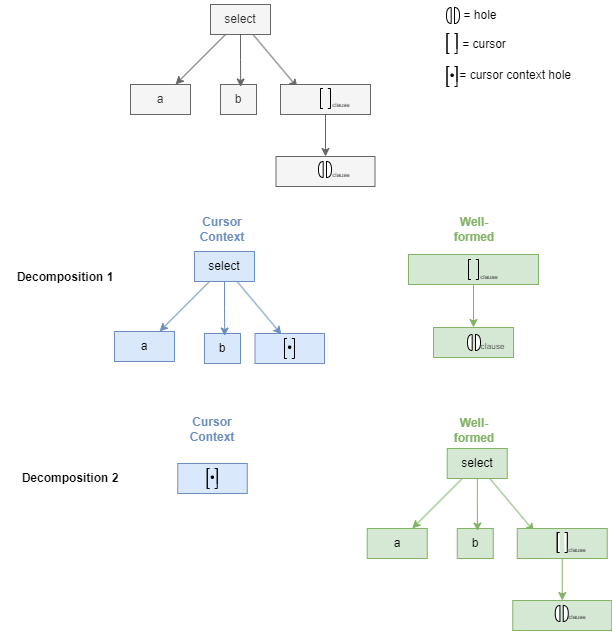
\includegraphics[width=\textwidth]{img/slq-decompose-ex.drawio.png}
  \caption{Two different decompositions of the same term}
  \label{fig:sql-decomp-ex}
\end{figure}

Decomposition should be generic and be possible on a valid abt of any given syntax.
For this we have a typeclass called \texttt{decomposable} that contains a
method called \texttt{decompose} which takes a statement made up by the
operators of sort $\mathcal{S}$, and returns a cursor-context and well-formed-tree pair,
if decomposition is possible.

In order to instantiate the \texttt{decomposable} type class for any sort,
it is then necessary to specify how we for any term in any sort,
can decompose uniquely into a cursor context and well-formed-tree pair.

Unique decomposition of an abt can be defined algorithmically and divided
into following sub-tasks:
\begin{itemize}
  \item Locate the cursor in the tree to be decomposed and generate a path to the cursor
  \item Generate an abt of sort $s^C \in \mathcal{S}^C$ based on the cursor path
  \item Generate an abt of sort $\dot{s} \in \dot{\mathcal{S}}$
        based on the rest of the tree that was not traversed
        when generating the cursor context
\end{itemize}

The following will explain in more details how the steps above can be done,
and how we always get a unique decomposition, as long as the abt to be decomposed is well-formed.

\subsubsection{Cursor path}

Generating a path to the cursor in the abt of sort $s \in \mathcal{S}$ extended with
hole and cursor operators (\cref{def:base-as})
simplifies the process of generating the cursor context. The path tells us
which operator $o^C \in \mathcal{O}^C$ replaces each $o \in \mathcal{O}$.
The list can be generated by performing pre-order traversal of the tree to be decomposed,
extending the list with every $i$, representing which argument in an operator of
arity $(\vec{s}_1.s_1, ... , \vec{s}_i.s_i, ..., \vec{s}_n.s_n)\mathcal{S}$ was
followed to locate the cursor. See \cref{lst:cursor-path-pseudocode} for pseudocode
demonstrating this process.

\begin{lstlisting}[caption={Pseudocode for generating cursor path},label={lst:cursor-path-pseudocode},
  style=inline]
getCursorPath op path =
  case op of
    cursor -> path
    _ -> 
      case length op.arity of
        0 -> []
        _ -> 
          map ++ 
            (index_map 
              (\i child -> 
                getCursorPath child (path ++ [i])) 
            op.arity)

\end{lstlisting}

The implementation of such a function depends on the set of sorts $\mathcal{S}$
and arity-indexed family of operators $\mathcal{O}$ given by the abstract syntax
of a language. The Elm CodeGen package\cite{elm-codegen-package} has been used to
generate a \texttt{getCursorPath} function for a \texttt{Base} type (\cref{lst:cursor-path-fun-gen}).
The function makes use of the helper function
\texttt{getBranchList} which is left out for brevity, but its purpose is
to generate a case expression for every syntactic category in the given syntax.
See \cref{ex:cursor-path-c} for an excerpt of the generated \texttt{getCursorPath}
function for the small C language (\cref{ex:c-spec}).

\begin{lstlisting}[language=elm,style=inline,caption={getCursorPath function generator},label={lst:cursor-path-fun-gen}]
createGetCursorPath : Syntax -> Elm.Declaration
createGetCursorPath syntax =
    Elm.declaration "getCursorPath" <|
        Elm.withType
            (Type.function
                [ Type.list Type.int
                , Type.named [] "Base"
                ]
                (Type.list Type.int)
            )
            (Elm.fn2
                ( "path", Nothing )
                ( "base", Nothing )
                (\_ base ->
                    Elm.Case.custom base
                        (Type.named [] "Base")
                        (getBranchList syntax)
                )
            )    
\end{lstlisting}

\begin{example}{Generated cursor path finder function}{ex:cursor-path-c}
  Following is an excerpt of the generated \texttt{getCursorPath} function
  for the small C language:
  \begin{lstlisting}[language=elm,style=inline,backgroundcolor=\color{myexamplecolorback}]
getCursorPath : List Int -> Base -> List Int
getCursorPath path base =
  case base of
    P p ->
      case p of
        Program arg1 ->
          getCursorPath (path ++ [ 1 ]) (Fd arg1)

        Hole_p ->
          []

        Cursor_p _ ->
          path
    ...
    Vd vd ->
      case vd of
        Vardecl arg1 arg2 ( boundVars3, arg3 ) ->
          (getCursorPath
            (path ++ [ 1 ])
            (T arg1)
            ++ getCursorPath
                (path ++ [ 2 ])
                (E arg2)
          )
          ++ getCursorPath
              (path ++ [ 3 ])
              (Bi arg3)

        Hole_vd ->
          []

        Cursor_vd _ ->
          path
\end{lstlisting}

  Notable for this example is the \texttt{Vardecl} branch, which represents an
  operator with three arguments, hence the need for three recursive calls to
  \texttt{getCursorPath}. The third argument is deconstructed since it is a binder,
  although the bound variables are not used in the cursor path generation,
  as the cursor cannot be in a bound variable.

\end{example}


\subsubsection{Cursor context}

Having the cursor path, the cursor context can be generated by replacing every
operator $o \in \mathcal{O}$ with its corresponding cursor context operator
$o^C \in \mathcal{O}^C$, with respect to which argument in the operator was
followed to locate the cursor. This is also done by performing pre-order traversal
of the tree, but it will stop when the cursor is reached (i.e. when the
cursor path is empty) and replace the operator reached with the
context hole operator $[ \ \cdot \ ] \in C$. The rest of the tree which has not
been traversed will be passed to the next step, generating the well-formed tree.
See \cref{lst:cursor-ctx-pseudocode} for pseudocode demonstrating this process.

\begin{lstlisting}[caption={Pseudocode for generating cursor context}
  ,label={lst:cursor-ctx-pseudocode}
  ,style=inline
  ]
toCCtx op path =
  case path of
    [] -> (context_hole, op)
    pathi :: pathrest -> 
      case op of
        cursor -> error "invalid path"
        _ ->
          case length op.arity of
            0 -> error "invalid path"
            _ ->
              case pathi of
                1 ->
                  let (cctxarg1, restTree) = 
                      toCCtx op.args[1] rest
                  in
                    (Cctx1_opName cctxarg1
                    , restTree) 
                2 ->
                  let clessarg1 =
                      toCLess op.args[2]
                  let (cctxarg2, restTree) = 
                      toCCtx op.args[2] rest
                  in
                    (Cctx2_opName clessarg1 cctxarg2
                    , restTree)
                ...
toCLess op =
  case op of
    Cursor _ -> error "not wellformed"
    _ ->
      case length op.arity of
        0 -> CLess_opName
        1 -> CLess_opName 
                (toCLess op.args[1])
        2 -> CLess_opName 
                (toCLess op.args[1]) 
                (toCLess op.args[2])
\end{lstlisting}

Functions supporting this are generated by Elm CodeGen, and can be seen in
\cref{lst:to-cc-fun-gen}, where a \texttt{toCCtx} function is generated
for the \texttt{Base} type in conjunction with a
\texttt{toCCtx\_s} for every $s$ syntactic category in the given syntax, where
the algorithm described above is implemented for every sort.

\begin{lstlisting}[language=elm
    ,style=inline
    ,caption={toCCtx function generator}
    ,label={lst:to-cc-fun-gen}
    ]
createToCCtxFuns : Syntax -> List Elm.Declaration
createToCCtxFuns syntax =
  List.map createToCCtxFun syntax.synCatOps ++ 
  [ Elm.declaration "toCCtx" <|
    Elm.withType
      (Type.function
        [ Type.named [] "Base"
        , Type.list Type.int ]
        (Type.tuple 
          (Type.named [] "Cctx") 
          (Type.named [] "Base"))
      ) <|
      Elm.fn2
        ( "base", Nothing )
        ( "path", Nothing )
        (\base path ->
          Elm.Case.custom base
            (Type.named [] "Base")
            (List.map
              (\synCatOp ->
                Elm.Case.branchWith
                  synCatOp.synCat
                  1
                  (\exps ->
                    Elm.apply 
                      (Elm.val <|
                      "toCCtx_" ++ synCatOp.synCat) 
                      (exps ++ [ path ])
                  )
              )
              syntax.synCatOps
              )
        )
  ]
\end{lstlisting}

\subsubsection{Well-formed tree}

The well-formed tree is generated by performing pre-order traversal of the
rest of the tree that was not traversed when generating the cursor context.
This is done by first replacing the cursor with the well-formed operator
$\dot{o} \in \dot{\mathcal{O}}$ of arity $(\hat{s})\dot{s}$ indicating that the
cursor encapsulates the root of a cursorless abt of sort $\hat{s}$.
After this, the rest of the tree is traversed, and every operator $o \in \mathcal{O}$
is replaced with its corresponding cursorless operator $\hat{o} \in \hat{\mathcal{O}}$.
See \cref{lst:wf-tree-pseudocode} for pseudocode demonstrating this process.

\begin{lstlisting}[caption={Pseudocode for generating well-formed tree},label={lst:wf-tree-pseudocode}, style=inline]
toWellformed op =
  let op = consumeCursor op
  in
    case length op.arity of
      0 -> error "not wellformed"
      1 -> Cursor_opName
              (toCLess op.args[1])
      2 -> Cursor_opName
              (toCLess op.args[1])
              (toCLess op.args[2])
      ...

consumeCursor op =
  case op of
    Cursor under -> under
    _ -> op
\end{lstlisting}



Like when generating functions supporting cursor context, a very similar approach
is taken here, and can be seen in listing \cref{lst:to-wf-fun-gen}.

\begin{lstlisting}[language=elm
    ,style=inline
    ,caption={toWellFormed function generator}
    ,label={lst:to-wf-fun-gen}
    ]
createToWellFormedFun : Syntax -> Elm.Declaration
createToWellFormedFun syntax =
  Elm.declaration "toWellformed" <|
    Elm.withType 
      (Type.function 
        [ Type.named [] "Base" ] 
        (Type.named [] "Wellformed")) <|
      Elm.fn
          ( "base", Nothing )
          (\base ->
            Elm.Case.custom
                (Elm.apply 
                  (Elm.val "consumeCursor") 
                  [ base ])
                (Type.named [] "Base")
                (List.map
                  (\synCatOp ->
                    branchWith synCatOp.synCat
                        1
                        (\exps ->
                          Elm.apply
                              (Elm.val <| 
                                "Root_" ++ 
                                synCatOp.synCat ++ 
                                "_CLess")
                              [ Elm.apply 
                                (Elm.val <| 
                                  "toCLess_" ++ 
                                  synCatOp.synCat) 
                                exps 
                              ]
                        )
                  )
                  syntax.synCatOps
                )
          )
\end{lstlisting}

The cursor context and well-formed tree pair as defined above will decompose
any well-formed abt into a unique pair of a cursor context and a well-formed tree.


\subsubsection{Cursor movement}
Cursor movement is a fundamental operation, allowing the editor to move the cursor
to a different position, changing the target of editor expressions. This is defined
as two operations in the editor calculus\cite{aalborg} in the form of
\texttt{Child-i} and \texttt{Parent} operations (\cref{fig:red-rules-movement}).

For moving to child $i$ of an operator, a \texttt{child} function is generated
which takes an integer $i$ and a decomposed tuple of a cursor context and well-formed
tree. It returns a new tuple, where the context hole in the cursor context has been 
replaced with the operator of sort $\mathcal{S}^C$ corresponding to the cursorless
operator of sort $\hat{\mathcal{S}}$ under the cursor in the well-formed tree before
moving the cursor. The integer $i$ determines which argument of the cursor context 
operator contains the new context hole. The new well-formed tree is built by 
wrapping the $i$ argument of the cursorless operator current root operator 
in the well-formed tree. 

For a visualization of this, see \cref{fig:cursor-movement-drawing}.

\begin{figure}[H]
  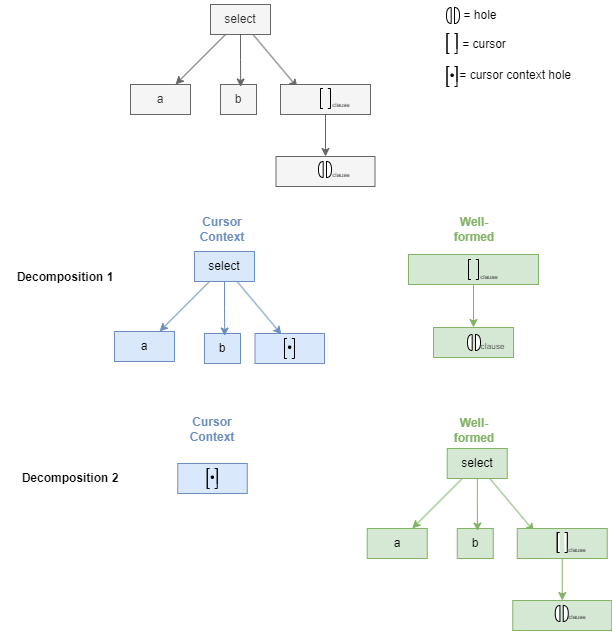
\includegraphics[width=\textwidth]{img/slq-decompose-ex.drawio.png}
  \caption{TODO}
  \label{fig:cursor-movement-drawing}
\end{figure}

\subsubsection{Substitution}
Substitution allow for replacing the abt encapsulated by the cursor with another
abt of the same sort, ensuring that well-formedness is maintained.
This is defined as the \texttt{Insert-op} operation in the editor calculus
(\cref{fig:red-rules-sub}).

For this a \texttt{substitution} function is generated 

\subsubsection{Conditional expressions}
Conditional expressions provide a way to perform different operations based on
modal logic of the encapsulated abt, such as the $@o$ operator which holds
if the cursor is encapsulating the operator $o$. This is defined as \texttt{At-op}
along \texttt{Necessity}, \texttt{Possibly-i} and \texttt{Possibly-i} operators
in the editor calculus\cite{aalborg} (\cref{fig:sat-rel-modal-ops}). Conditionals
can be connected with logical operators, forming the operators \texttt{Negation},
\texttt{Conjunction}, \texttt{Disjunction-1} and \texttt{Disjunction-2}
(\cref{fig:sat-rel-prop-connectives}).





\subsubsection{Making the functionality generic}
% TODO: write a smooth transition

For example, consider the cursor substitution operator (\cref{fig:red-rules-sub}),
where the editor calculus enforces that operators can only be substituted
with operators of same sort. Initially, a straightforward approach involves
having a substitution function for each sort $s \in \mathcal{S}$.
This approach of course leads an implementer to consider generalization,
i.e. how a single function can take any cursor-encapsulated abt and replace it
with an operator of the same sort. A solution to this could be
% % TODO: replace this with a more interesting example, i.e. conditionals
using type classes, where we might have a type class called \texttt{substitutable}
and having an instance for each sort.
Having a typeclass is possible in Haskell (\cref{lst:haskell-typeclass}),
but typeclasses are not directly supported by Elm.
They can however be simulated with Elm records, as shown in the "typeclasses"
Elm package\cite{elm-typeclass-package}.
An example of such a simulation is shown in \cref{lst:elm-typeclass}.
This typeclass simulation in Elm has the disadvantage of forcing an explicit
reference to the typeclass "instance" in a generic function, in contrast to Haskell.
This leads to more verbose code and more source code generation.

% TODO: replace this with a more interesting example, i.e. conditionals
\begin{lstlisting}[language=Haskell,style=inline,caption={Haskell typeclass example},label={lst:haskell-typeclass}]
-- typeclass
class Substitutable a where 
    substitute :: a -> a -> a
    
-- instance of typeclass
instance Substitutable a where
    substitute _ replacement = replacement

-- example usage
doIntSub :: Int
doIntSub = substitute 1 2 
\end{lstlisting}


% TODO: replace this with a more interesting example, i.e. conditionals
\begin{lstlisting}[language=elm,style=inline,caption={Elm typeclass simulation example},label={lst:elm-typeclass}]
{-| Simulate a type class
-}
type alias Substitutable a =
    { substitute : a -> a -> a }

{-| Generic instance of the typeclass, we don't need any specific implementation for each type/sort, we just want to assure that the expression and replacement are of the same type. This is constrained by the `substitute` function signature in the (simulated) typeclass.
-}
substituteAny : Substitutable a
substituteAny =
    { substitute = \_ replacement -> replacement }

{-| Polymorphic function that can be used with any type that has an instance of the `Substitutable` typeclass.
-}
substitute : Substitutable a -> a -> a -> a
substitute substitutable expression replacement =
    substitutable.substitute expression replacement

{-| Example usage
-}
doIntSub : Int
doIntSub =
    substitute substituteAny 1 2
\end{lstlisting}